Similar to the loop bound computation,
we first compute two abstract states for each loop w.r.t. a simple transition path inside it,
$\lpinit(l: \rprog, \tpath, c)$, and $\lpnext(l: \rprog, \tpath, c)$ based on the refined program
as in Definition~\ref{def:alg-absstate}.
\begin{defn}[Loop Abstract States]
\label{def:alg-loopabsstate}
Given a program $c$ with its refined program $\rprog_c$ and a loop sub-program  and $l:\rprog$ in $\rprog_c$,
we compute four two abstract states for the ranking functions in this loop, 
   $\lpinit(l: \rprog, \tpath, c)$, and $\lpnext(l: \rprog, \tpath, c) \in \scexpr(c)$ as follows.
   \begin{itemize}%
   \item 
The loop initial state 
$\lpinit(l: \rprog, \tpath, c) \in \scexpr(c)$ computes a symbolic expression estimating the abstract initial value of $\tpath$'s ranking function before
any visit of $\tpath$ and during the first execution of $l: \rprog$.
\[
  \begin{array}{l}
    \lpinit(l: \rprog, \tpath, c) \triangleq 
  \arg\max_{l_1}
  \\
  \left\{
       \varinvar(y, c) + v ~\middle\vert~ 
       \begin{array}{l} 
         (l_1, x' \leq y + v, l_2) \in \reset(x, c) 
         \\
         \land \absinit(\rprog) \leq l_1 \leq \absinit(\tpath)
         \land
         x \in \left\{ \locbound(\absevent, c) | \absevent \in \tpath \right\}
       \end{array}
     \right\}
    \end{array}
    \]
\item
The loop next state 
$\lpnext(l: \rprog, \tpath, c) \in \scexpr(c)$ 
computes the amount of $\tpath$'s ranking function
that is is modified before
the second visit of $\tpath$ but during the second execution of $l: \rprog$.
$ 
\lpnext(l: \rprog, \tpath, c) \triangleq 
\max\limits_{x \in \left\{ \locbound(\absevent, c) | \absevent \in \tpath \right\}}
$
%
{\small
\[
  \begin{array}{l}
  % \lpnext(l: \rprog, \tpath, c) \triangleq 
  % \max\limits_{x \in \left\{ \locbound(\absevent, c) | \absevent \in \tpath \right\}}
  % \\
  \left\{
    \begin{array}{l}
  \sum\limits_{\absevent \in \inc(x, c) }
  \left\{ 
      v ~\middle\vert~ \absevent = (l', x' \leq x + v, \_) \land  l' \in \rprog 
      \land l' \notin \tpath \right\}
      \\ \qquad 
      + \arg\max\limits_{l_2 }
         \left\{ \varinvar(y, c) + v ~\middle\vert~ 
         (l_1, x' \leq y + v, l_2) \in \reset(x, c) \land l_1 \in \rprog \land l_1 \notin \tpath\right\}
     \\ \qquad 
      - \sum\limits_{ \absevent \in \dec(x, c) }\left\{ 
      v 
      ~\middle\vert~ \absevent = (l', x' \leq x + v, \_) \land l' \in \rprog \land l' \notin \tpath \right\}
      \\ \qquad 
      + BD(\kw{enclosed}(\tpath), c) \times \rfnext(\tpath, c)
    \end{array}
    \right\}
  \end{array}
  \]
  }
    \end{itemize}
\end{defn}
%
Then we compute the
\emph{loop reachability-bound} as below.
% using the two states and the $\rffinal$.
\begin{defn}[Loop Reachability-bound Computation]
  \label{def:looprb}
  Given a refined program $\rprog$ and a simple transition path $\tpath$ in this program, 
  let $l: \rprog_l$ be a loop program in $\rprog$,
  then $l: \rprog_l$'s \emph{loop reachability-bound} w.r.t. $\tpath$, $\lpchB(l: \rprog, \tpath, c)$
  is computed interactively with the abstract loop states as follows. 
  \[
    \lpchB(l: \rprog, \tpath, c) \triangleq
    \max\limits_{x = a \in \rffinal(\tpath, c)}
    \frac{\lpinit(\rprog, \tpath, c) - a }{\lpnext(\rprog, \tpath, c)}
  \]
\end{defn}
%
Again in Example~\ref{ex:relatedNestedWhileOdd-overview}, $\tpath_3$ has an outer loop program $\rprog_1^1$.
We first compute $\lpinit(\rprog_1^1, \tpath_3, c) = n - m $ and $\lpnext(\rprog_1^1, \tpath_3, c) = n - m - 1$ and then derive $\lpchB(\rprog_1^1, \tpath_3, c) = 1$ as tight as expected.
%

We also guarantee the soundness of \emph{loop reachability-bound} in \highlight{Appendix~\ref{apdx:looprb-sound}}.
The $\lpchB(l:\rprog, \tpath)$ 
can also be over-approximated by
$I(l, l')$ through the progress invariant in paper\cite{GulwaniJK09}.
While $I(l, l')$ over-approximates this value largely
by estimating the bound on iteration numbers of $l'$ in one iteration of $l$.

Example~\ref{ex:relatedNestedWhileOdd-overview} has only two level nested loop, and
the only interesting \emph{loop reachability-bound} are $\lpchB(\rprog_1^1, \tpath_3)$.
We illustrate Example~\ref{ex:threeNestedWhile} with three nested loops, which can better show the improvement of the \emph{loop reachability-bound}.
\begin{example}[Three Nested Loop]
  \label{ex:threeNestedWhile}
    %
    \begin{figure}
    \centering
    %
    \vspace{-0.8cm}
    \begin{subfigure}{.45\textwidth}
        $
        \begin{array}{l}
            N < m < n\\
            \kw{threeNestedWhile}(n, m, N) \triangleq \\
            \clabel{ \assign{i}{0} }^{0} ; \\
                L_1: \ewhile ~ \clabel{i < n}^{1} ~ \edo ~ \\
                \quad (
                 \highlight{\clabel{\assign{j}{0}}^{2}} ;\\
                 L_3:  \quad \ewhile ~ \clabel{j < m}^{3} ~ \edo ~ \\
                \quad \quad ( \clabel{\assign{j}{j+1}}^{4};\\
                  \quad \quad \highlight{\clabel{\assign{w}{i}}^{5}};\\
                  L_6:  \quad \quad \ewhile ~ \clabel{w < N}^{6} ~ \edo ~ \\
                  \quad \quad \quad ( \clabel{\assign{w}{w + 1}}^{7} ); \\
                      \quad \quad \clabel{\assign{i}{w}}^{8}
                      ); \\
                      \quad \clabel{\assign{i}{i+1}}^{9})
            \end{array}
            $
            \vspace{-0.2cm}
            \caption{}
        \end{subfigure}
    \begin{subfigure}{.48\textwidth}
        \begin{centering}
            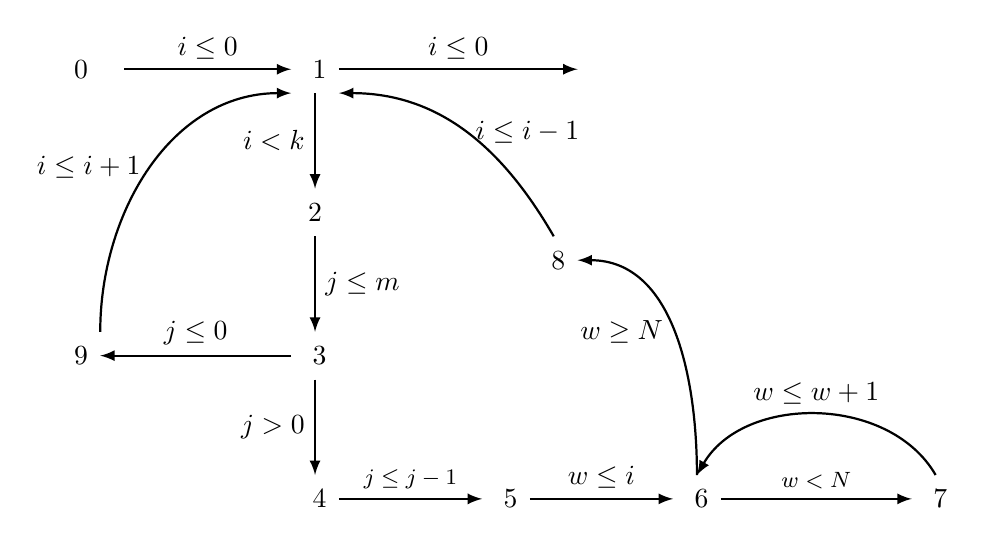
\begin{tikzpicture}[scale=\textwidth/20cm,samples=200]
                \draw[] (-5, 10) circle (0pt) node{{ $0$}};
                \draw[] (0, 10) circle (0pt) node{{ $1$}};
                \draw[] (6, 10) circle (0pt) node {{$\lex$}};
                \draw[] (0, 7) circle (0pt) node{{$2$}};
                \draw[] (0, 4) circle (0pt) node{{ $3$}};
                \draw[] (-5, 4) circle (0pt) node{{ $9$}};
                \draw[] (0, 1) circle (0pt) node{{ $4$}};
                \draw[] (4, 1) circle (0pt) node{{ $5$}};
                \draw[] (8, 1) circle (0pt) node{{ $6$}};
                \draw[] (13, 1) circle (0pt) node{{ $7$}};
                \draw[] (5, 6) circle (0pt) node{{ $8$}};
                % Counter Variables
                %
                % Control Flow Edges:
                \draw[ thick, -latex] (-4, 10)  -- node [above] {$i \leq 0$}(-0.5, 10);
                \draw[ thick, -latex] (0, 9.5)  -- node [left] {$i < k$} (0, 7.5) ;
                \draw[ thick, -latex] (0, 6.5)  -- node [right] {$j \leq m$} (0, 4.5) ;
                \draw[ thick, -latex] (0, 3.5)  -- node [left] {$j > 0$} (0, 1.5) ;
                \draw[ thick, -latex] (-0.5, 4)  -- node [above] {$j \leq 0$} (-4.5, 4) ;
                \draw[ thick, -latex] (-4.5, 4.5)  to  [out=90,in=180]  node [left] {$i \leq i + 1$ }(-0.5, 9.5);
                \draw[ thick, -latex] (0.5, 10)  -- node [above] {$i \leq 0$}  (5.5, 10);
                \draw[ thick, -latex] (0.5, 1)  -- node [above] {{\footnotesize $j \leq j - 1$}}  (3.5, 1);
                \draw[ thick, -latex] (4.5, 1)  -- node [above] {$w \leq i$}  (7.5, 1);
                \draw[ thick, -latex] (8.5, 1)  -- node [above] {{\footnotesize $w < N$}}  (12.5, 1);
                \draw[ thick, -latex] (8, 1.5)  to [out=90,in=0] node [left] {{$w \geq N$}}  (5.5, 6);
                \draw[ thick, -latex] (13, 1.5)  to  [out=120,in=60] node [above] {$w \leq w + 1$}  (8, 1.5);
                \draw[ thick, -latex] (5, 6.5)  to  [out=120,in=0]  node [right] {$i \leq i - 1$ }(0.5, 9.5);
                \end{tikzpicture}
%     \caption{}
%     \end{centering}
%     \end{subfigure}
% \begin{subfigure}{.2\textwidth}    
% \begin{centering}
    {\small
$
    \begin{array}{ll}
        \tpath_0 = (0 \to 1)
        &
        \tpath_4 = (6 \to 8 \to 3)
        \\        
        \tpath_1 = (1 \to 2 \to 3)
        &
        \tpath_5 = (3 \to 9 \to 1)
        \\
        \tpath_2 = (3 \to 4 \to 5 \to 6)
        &
        \tpath_6 = (1 \to \lex)
        \\
        \tpath_3 = (6 \to 7 \to 6)
    \end{array}
$
}
\vspace{-0.2cm}
\caption{}
\end{centering}
\end{subfigure}
% $
%     \begin{array}{l}
%         \rprog_1 = {\rprepeat(\tpath_1; 3: {\rprepeat(\tpath_2; 6 : {\rprepeat(\tpath_3)}; \tpath_4)}; \tpath_5)}
%         \\
%         \rprog_3 = {\rprepeat(\tpath_2; 6 : {\rprepeat(\tpath_3)}; \tpath_4)}
%     \end{array}
% $
$\rprog = \tpath_0; 1: \rprepeat(\tpath_1; 3: {\rprepeat(\tpath_2; 6 : {\rprepeat(\tpath_3)}; \tpath_4)}; \tpath_5);\tpath_6$
\vspace{-0.2cm}
\caption{
    (a) An example of three nested loops with related iterators,
    (b) the abstract transition graph, simple transition paths and loop body.}
    \vspace{-0.8cm}
        \label{fig:threeWhile-overview}
    \end{figure}
This example is similar to the loop $L_4$ nested in the second branch in example~\ref{ex:relatedNestedWhileOdd-overview}.
$w$ is reset by $j$ in command 5 and $i$ is then reset by $w$, so $L_6$ is only executed in the first iteration of loops $L_1$ and $L_3$.
% \\
Then the total iterations times are
$n + m^2 - m \times N$,
and the expected \emph{reachability-bound} for location $7$ inside the $L_6$ is $N$,
for locations $4, 5$ and $8$ between the $L_3$ and $L_6$ are $(n-N) \times (m - N)$,
and $n - N$ for locations $2$ and $9$.
% \\
The challenge here is that the locations inside the loop $L_6$ has the same
$\psRB$ as loop iteration times of $L_6$.
% , as well as our \emph{path reachability-bound}.
However, the locations between $L_3$ and $L_6$'s $\psRB$ are the multiplication of the inner and outer loop iteration bounds.
In order to precisely compute their $\psRB$, it is critical to know
the numbers of iterations of the outside loop $L_3$ and $L_1$ such that,
during these iterations, the loop $L_6$ is ``entered'', which is exactly our \emph{loop reachability-bound}.

Figure~\ref{fig:threeWhile-overview}(a) shows its abstract transition graph,
and we compute its refined program in the bottom of Figure~\ref{fig:threeWhile-overview}. 
We first compute the $\outinB(\tpath_3, \rprepeat(\tpath_3)) = N $ for $\tpath_3$ w.r.t. its innermost loop.
Since $\tpath_3$ has two outer loops, $L_1$ and $L_3$.
%  it is nested.
To compute $\lpchB(3: \rprog_3, \tpath_3)$, where we use $\rprog_3$ denotes the body of the loop $L_3$,
we first compute $\lpinit( \rprog_1, \tpath_3, c) = 0$,
$\lpnext( \rprog_1, \tpath_3, c) =  N + 1 $, and
$\rffinal(\rprog_1, c) = \{ i = n, k = N \}$.
So we can know $\lpchB(1: \rprog_1, \tpath_3, c) = \max\{ \frac{n - 0}{n - N - 1}, \frac{N - 0}{N +  1}\} = 1$, as expected.
\end{example}
